% Build: latexmk -pdf main.tex   (limit: 4 pages including figures)
\documentclass[10pt,letterpaper]{article}
\usepackage[margin=0.6in,top=0.5in,bottom=0.55in]{geometry}
\usepackage[T1]{fontenc}
\usepackage{lmodern}
\usepackage{microtype}
\usepackage{graphicx}
\usepackage{booktabs}
\usepackage{tabularx}
\usepackage{amsmath}
\usepackage{xcolor}
\usepackage{enumitem}
\usepackage{caption}
\usepackage{subcaption}
\usepackage{float}
\usepackage{listings}
\usepackage{tikz}
\usetikzlibrary{positioning,arrows.meta,fit}
\usepackage[hidelinks]{hyperref}
\hypersetup{pdftitle={Melchior Portfolio}, pdfauthor={Robert Everitt}}
\usepackage{titlesec}

\definecolor{accent}{HTML}{1F4E79}
\definecolor{codebg}{HTML}{F4F6F8}
\titleformat{\section}{\large\bfseries\color{accent}}{\thesection}{0.6em}{}
\titlespacing*{\section}{0pt}{7pt}{3pt}
\titleformat{\subsection}{\normalsize\bfseries}{\thesubsection}{0.5em}{}
\titlespacing*{\subsection}{0pt}{5pt}{2pt}
\setlist{nosep,leftmargin=1.2em}
\captionsetup{font=small,labelfont=bf,skip=3pt}
\setlength{\parskip}{3pt}
\setlength{\parindent}{0pt}
\setlength{\textfloatsep}{8pt}
\setlength{\intextsep}{6pt}
\lstset{basicstyle=\ttfamily\scriptsize,backgroundcolor=\color{codebg},
  frame=none,columns=fullflexible,keepspaces=true,showstringspaces=false,
  language=C,keywordstyle=\color{accent}\bfseries,commentstyle=\color{gray}}

\begin{document}

%-------------------------------------------------------------------------------
\begin{center}
{\LARGE\bfseries\color{accent} Melchior: Rocket Avionics Flight Data Recorder}\\[2pt]
{\large Custom avionics hardware, board bring-up, and embedded C drivers}\\[3pt]
\textbf{Robert Everitt} \textperiodcentered{} Solo project, June 2026 -- present \textperiodcentered{}
Developed for MASA-Dearborn rocketry\\[1pt]
\href{mailto:bobev@umich.edu}{\texttt{bobev@umich.edu}}
\end{center}
\vspace{-4pt}

%-------------------------------------------------------------------------------
\section{Overview and Motivation}
Melchior is a 4-layer STM32H5 flight computer I designed to log inertial and barometric data on high-power rockets, 
starting with my Level~2 certification flight on an AeroTech J270 solid propellant motor. Its job is to record low-latency sensor data for developing and testing state estimation algorithms. The overarching goal is to provide an iterative step towards a final board which is capable of deploying parachutes and lighting a sustainer solid propellant motor in flight.

\subsection{Why build it?} As a member of several engineering teams for the past six years, and as MASA-Dearborn's electrical lead in 2025, I have observed two recurring problems on the projects I have been a part of: 

\begin{enumerate}[leftmargin=1cm]
  \item systems too complex to develop in the course of a year, making it hard to do iterative testing
  \item projects which are scoped too large to hand off to new members
\end{enumerate}
Melchior is meant to be small, cheap, and easy to understand so it can be verified piece by piece, and new members can use it beyond my time on the team.

\subsection{My Role} I am handling development and testing of the entire system, from board routing, embedded system design, and sensor fusion algorithms, all the way to rocket construction and simulation. 
The goal is that after this academic year, the board can be used to teach future members, and gather sensor data for Kalman filter tuning.

%-------------------------------------------------------------------------------
\section{Requirements and System Architecture}
\begin{minipage}[t]{0.50\textwidth}
\vspace{0pt}
\small
\begin{tabularx}{\linewidth}{@{}lX@{}}
\toprule
\textbf{ID} & \textbf{Requirement (abridged)} \\
\midrule
R1 & Log IMU, barometer and magnetometer data at high rate ($>$100~Hz) to on-board flash. \\
R2 & Store full flight with room for error if parachutes deploy early, targeting a margin $3\times$ the 140~s simulated flight, $\geq 420$~s. \\
R3 & Measure beyond $\pm$16~g for boost and recovery shock events. \\
R4 & Robust error handling, ensuring the board is capable of recording data even in cases of individual sensor failure. \\
R5 & Estimate attitude \& altitude on board for post-flight algorithm comparison. \\
R6 & No pyro/actuation on this board; isolate safety-critical functions. \\
R7 & Debuggable without extra hardware: SWD, SWO trace, test points. \\
\bottomrule
\end{tabularx}
\end{minipage}\hfill
\begin{minipage}[t]{0.47\textwidth}
\vspace{0pt}
\centering
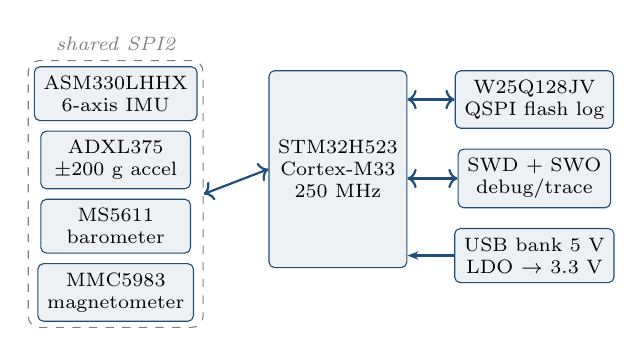
\begin{tikzpicture}[font=\scriptsize,
  blk/.style={draw=accent,fill=accent!8,rounded corners=2pt,minimum height=0.55cm,
              minimum width=1.9cm,align=center},
  arr/.style={-{Stealth[length=4pt]},thick,accent}]
\node[blk,minimum height=2.5cm,minimum width=1.7cm] (mcu) {STM32H523\\Cortex-M33\\250 MHz};
\node[blk,left=0.9cm of mcu.north west,anchor=north east,yshift=0.05cm] (imu) {ASM330LHHX\\6-axis IMU};
\node[blk,below=0.12cm of imu] (adxl) {ADXL375\\$\pm$200 g accel};
\node[blk,below=0.12cm of adxl] (baro) {MS5611\\barometer};
\node[blk,below=0.12cm of baro] (mag) {MMC5983\\magnetometer};
\node[blk,right=0.6cm of mcu.north east,anchor=north west] (flash) {W25Q128JV\\QSPI flash log};
\node[blk,below=0.25cm of flash] (dbg) {SWD + SWO\\debug/trace};
\node[blk,below=0.25cm of dbg] (pwr) {USB bank 5 V\\LDO $\to$ 3.3 V};
\node[draw=gray,dashed,rounded corners,fit=(imu)(mag),inner sep=2pt,
      label={[font=\scriptsize\itshape,gray]above:shared SPI2}] (bus) {};
\draw[arr,<->] (bus.east) -- (mcu.west);
\draw[arr,<->] (mcu.east |- flash) -- (flash.west);
\draw[arr,<->] (mcu.east |- dbg) -- (dbg.west);
\draw[arr] (pwr.west) -- (mcu.east |- pwr);
\end{tikzpicture}
\captionof{figure}{System block diagram.}
\end{minipage}

\vspace{4pt}
\textbf{Key trade-offs.}
\begin{itemize}
\item \textbf{MCU:} STM32H523 for its OCTOSPI peripheral (quad-SPI flash logging), DMA,
  floating-point unit, with pinout room for CAN later if board-to-board communication is desired. Published
  embedded UKF/EKF implementations ran acceptably on weaker cores, so 250~MHz was judged sufficient.
\item \textbf{Sensors:} chosen for high output data rate and vibration tolerance. The ASM330LHHX
  (automotive-grade, up to 6.7~kHz ODR) is the primary IMU; the ADXL375 covers up to $\pm$200~g (R3).
\item \textbf{Storage budget (R2):} one frame is 11 channels $\times$ 32 bits $= 44$ bytes. A 128~Mbit
  device holds $16{,}777{,}216 / 44 \approx 381{,}000$ frames: $\approx 61$~min at the current
  104~Hz rate, but only $\approx 381$~s at 1~kHz, short of R2. This sets a $\approx 900$~Hz ceiling on
  full-frame logging on the W25Q128JV. The same footprint supports flash chips up to 4$\times$ the size if higher data rate logging is desired.
\item \textbf{Power:} a USB power bank feeding an AMS1117 LDO, deliberately simple so power is not
  a variable while the logging system is proven. Battery protection and a buck are planned for testing in conjunction with the pyro channel circuitry on a separate board.
\end{itemize}

%-------------------------------------------------------------------------------
\section{Hardware Design}
\begin{figure}[H]
\centering
\begin{subfigure}[t]{2.89in}\centering
  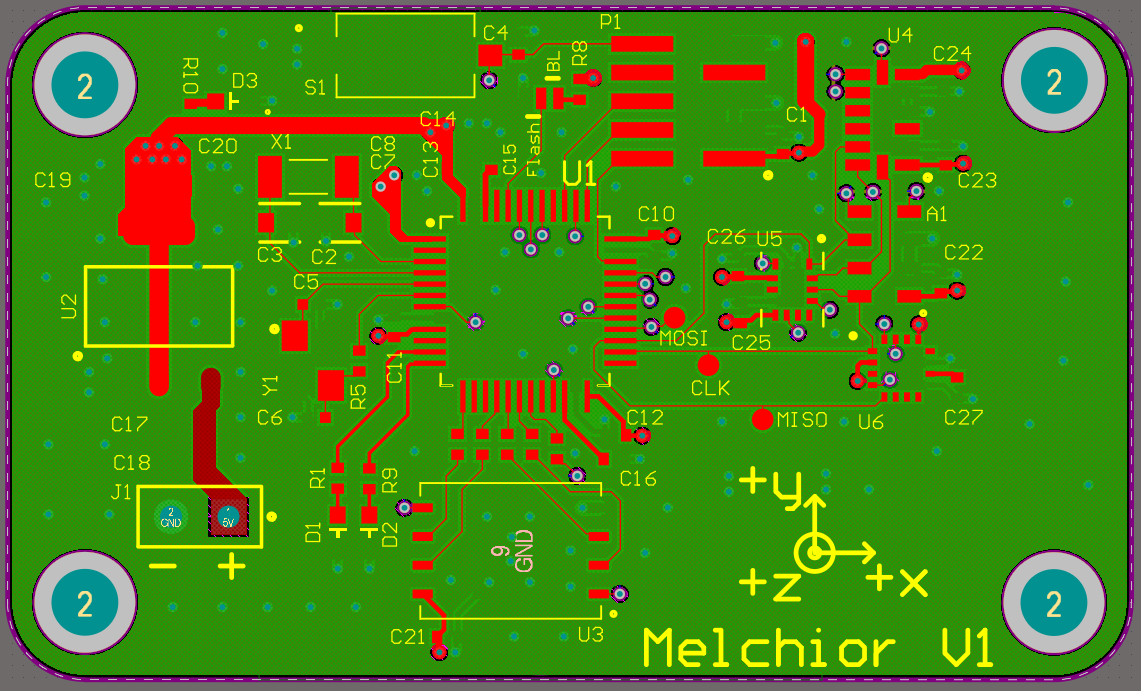
\includegraphics[height=1.75in]{figs/board_routed.png}
  \caption{Layout render (sensor cluster right, flash bottom).}
\end{subfigure}\hfill
\begin{subfigure}[t]{2.05in}\centering
  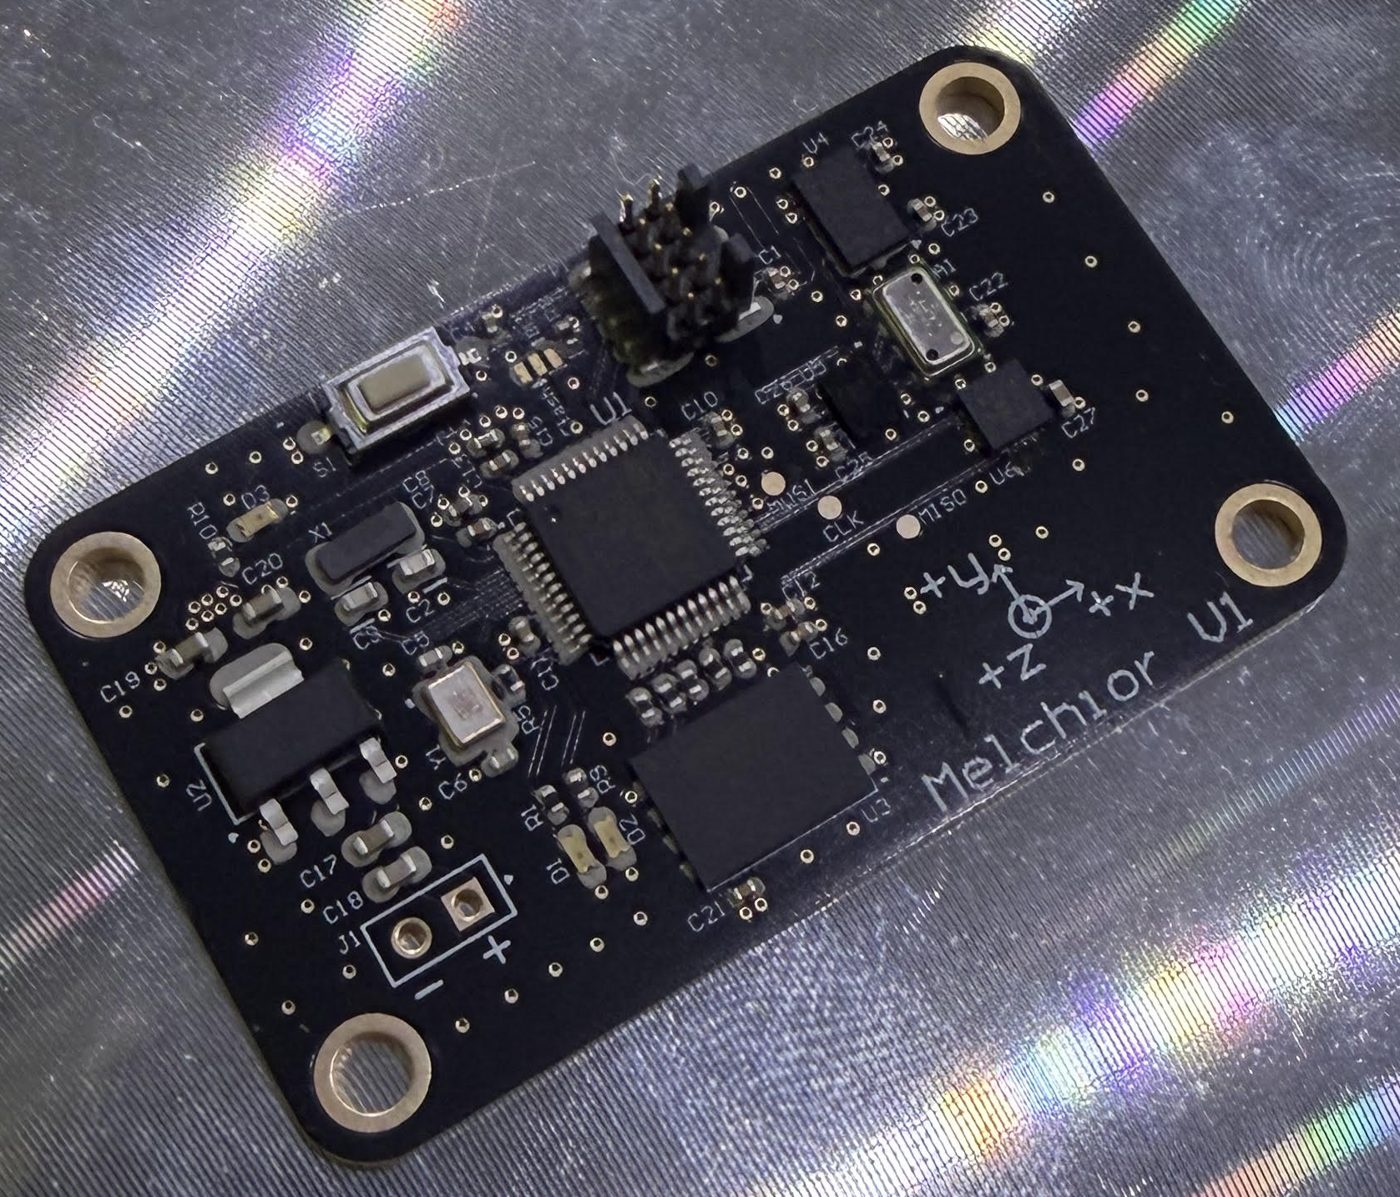
\includegraphics[height=1.75in]{figs/board_photo.jpg}
  \caption{Assembled Melchior V1.}
\end{subfigure}\hfill
\begin{subfigure}[t]{1.90in}\centering
  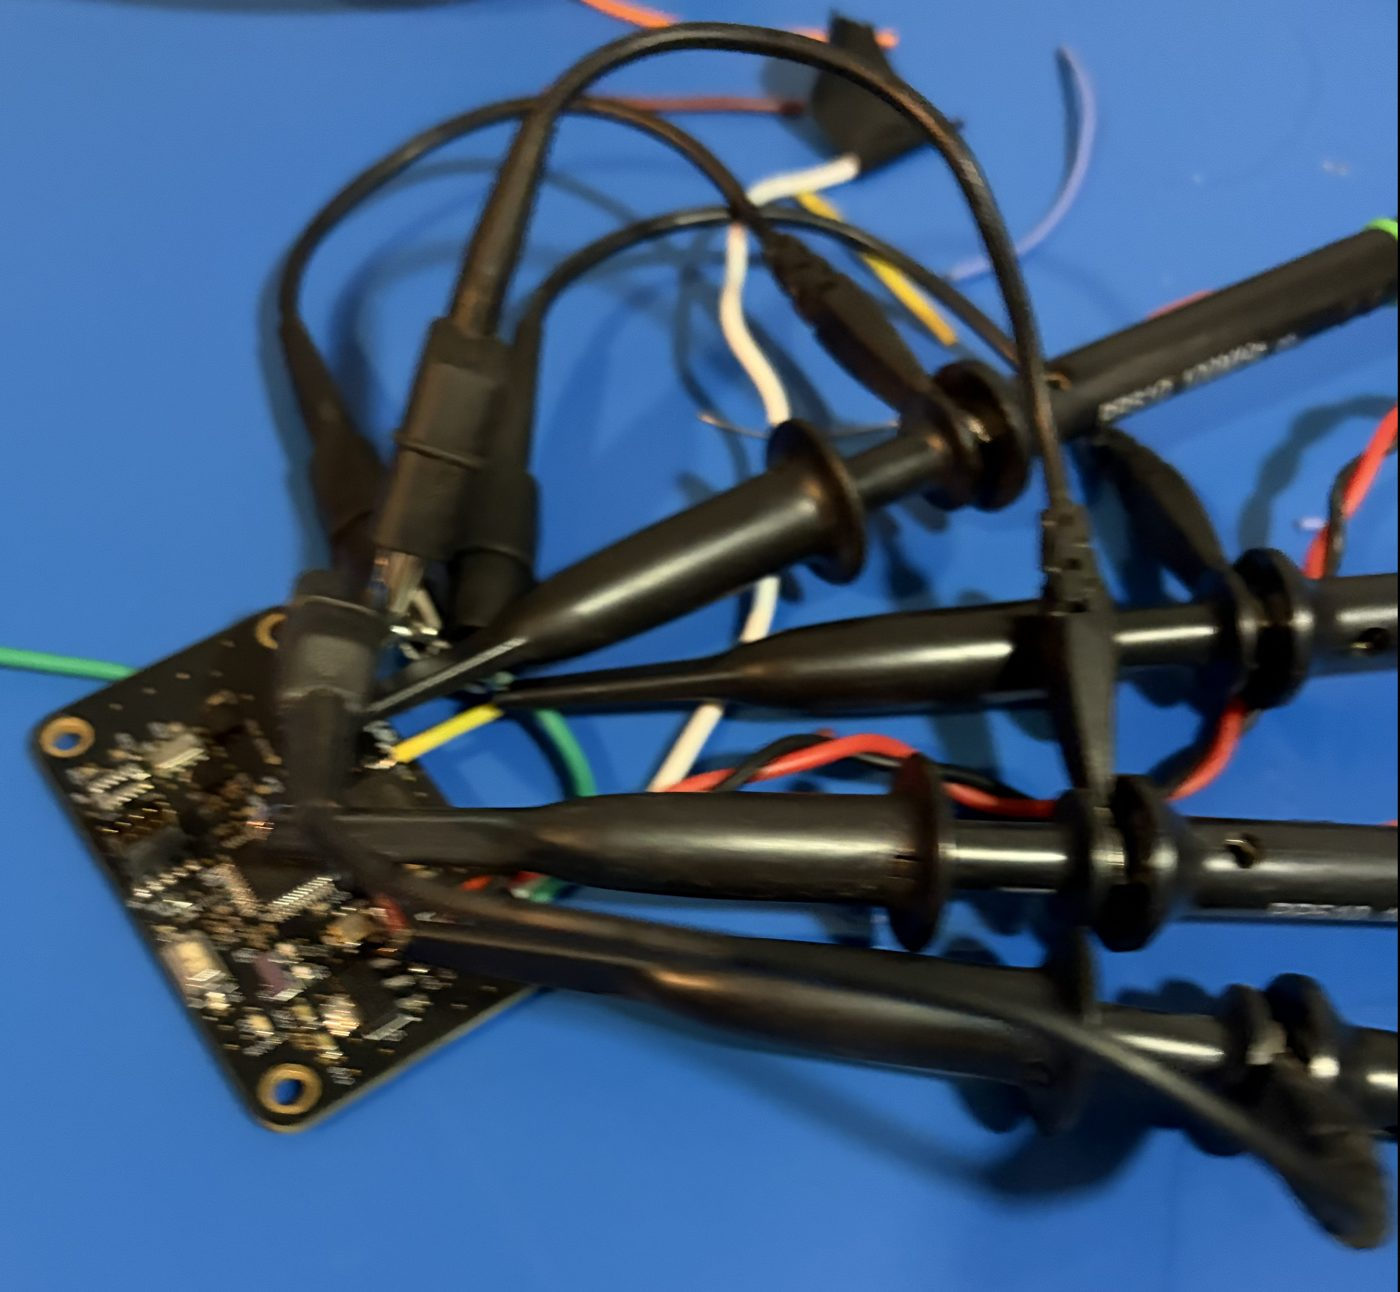
\includegraphics[height=1.75in]{figs/qspi_probe_setup.jpg}
  \caption{Probing QSPI lines.}
\end{subfigure}
\caption{Melchior V1 hardware.}
\end{figure}
\vspace{-4pt}
\begin{itemize}
\item \textbf{Stack-up:} Four layers with both internal layers as solid ground planes, with signals and
  power on the outer layers, giving every trace an unbroken return path next to it.
\item \textbf{Buses:} the four sensors share one SPI bus (individual chip selects; 5~MHz maximum, typically runs at 1.25~MHz for clock stability);
  the flash has a dedicated 4-bit QSPI bus with series resistors on CLK and IO0--IO3 to damp signal rise times.
\item \textbf{Debug-first design (R7):} 10-pin SWD header including SWO for tracing over ITM, SPI test points, status LEDs, a reset button, and a solder-jumper on BOOT0. Board axes are printed on the silkscreen so mounting orientation can be checked during integration.
\item \textbf{Real-time clock:} an RTC with a CR1616 backup cell timestamps sensor logs.
\end{itemize}

%-------------------------------------------------------------------------------
\section{Board Bring-up and Debugging}
I brought the board up one subsystem at a time (blinky $\to$ SWO $\to$ sensor IDs $\to$
measurements) to keep each failure's search space small. Three problems stood out:

\textbf{1. Firmware not starting after reflow.}
\begin{itemize}
\item \emph{Symptom:} SWD connected, but CubeIDE could not enter debug mode.
\item \emph{Diagnosis:} halting via ST-LINK/GDB showed a HardFault with PC at \texttt{0xEFFFFFFE}
  and invalid SP/LR, while VTOR pointed at the correct vector table. A valid image faulting at a
  nonsensical address implicated the boot path, not the application.
\item \emph{Fix:} the BOOT0 solder jumper had been left open; tying BOOT0 to ground made startup reliable.
\end{itemize}

\textbf{2. ADXL375 corrupting the shared SPI bus.}
\begin{itemize}
\item \emph{Symptom:} correct ID and data in isolation, but it could disrupt traffic to other sensors.
\item \emph{Diagnosis:} its CS pin also enables I\textsuperscript{2}C mode when high. In SPI mode~3
  SCLK idles high, so a MOSI edge during another sensor's transfer looks like an
  I\textsuperscript{2}C start condition, and the ADXL375 may drive the bus.
\item \emph{Fix:} part removed; a CS-gated SDA line is planned for rev~B. R3 stays open, but the
  ASM330LHHX at $\pm16$~g covers the J270's simulated 14.8~g peak.
\end{itemize}

\textbf{3. QSPI flash not responding.}
\begin{itemize}
\item \emph{Symptom:} a current-limited first power-up with a thermal camera caught the flash soldered
  backwards before it damaged power components. After hot-air rework, Read-ID (\texttt{0x9F}) still
  returned nothing instead of \texttt{EF 40 18}.
\item \emph{Diagnosis:} a firmware capture mode repeating only Read-ID let the scope trigger on CS.
  IO0 showed \texttt{0x9F} arriving; IO1 (flash data out) never toggled. All pads show continuity,
  so heat damage during rework is the working theory.
\item \emph{Next:} confirm with a replacement chip, now on order.
\end{itemize}

\textbf{Signal checks.} I also probed the QSPI clock at the flash and the sensor SPI clock at its
5~MHz limit (0--3.2~V, visibly rounded edges). All sensors communicate reliably; flight will run
at 1.25--2.5~MHz, with routing and setup/hold margin analysis on the rev~B checklist.

\begin{figure}[H]
\centering
\begin{subfigure}[t]{2.17in}\centering
  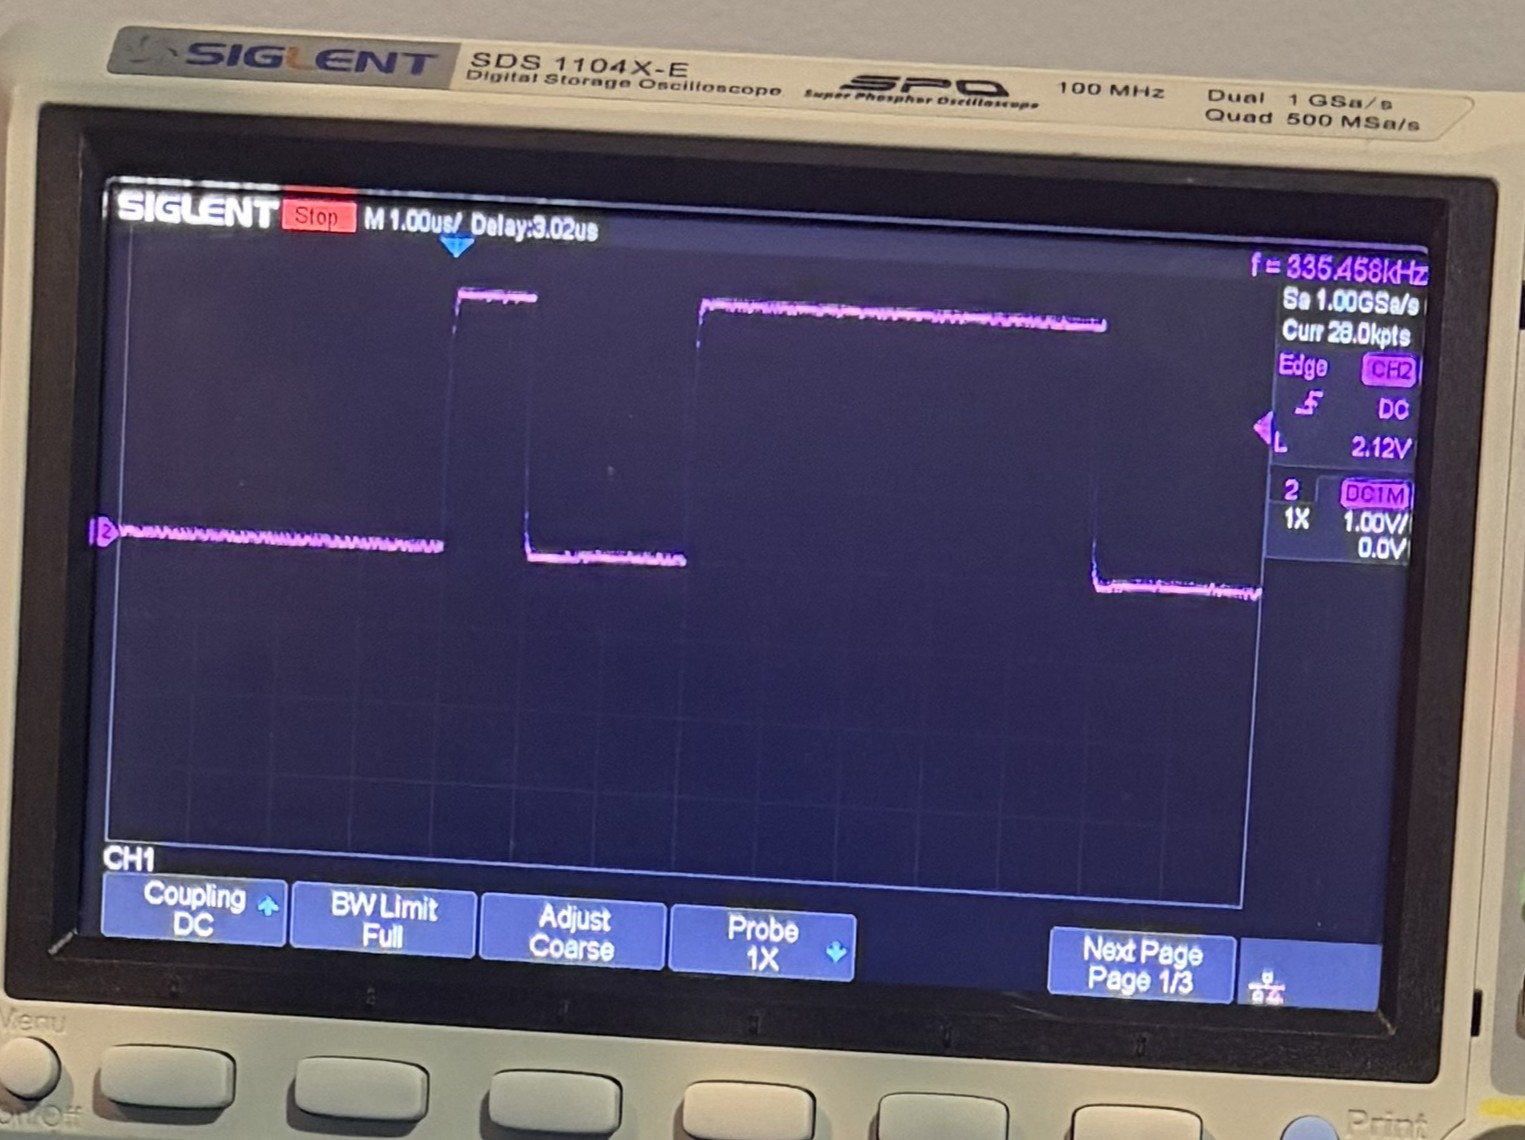
\includegraphics[height=1.62in]{figs/IMG_0650.jpeg}
  \caption{IO0 (MCU $\to$ flash) during Read-ID.}
\end{subfigure}\hfill
\begin{subfigure}[t]{1.89in}\centering
  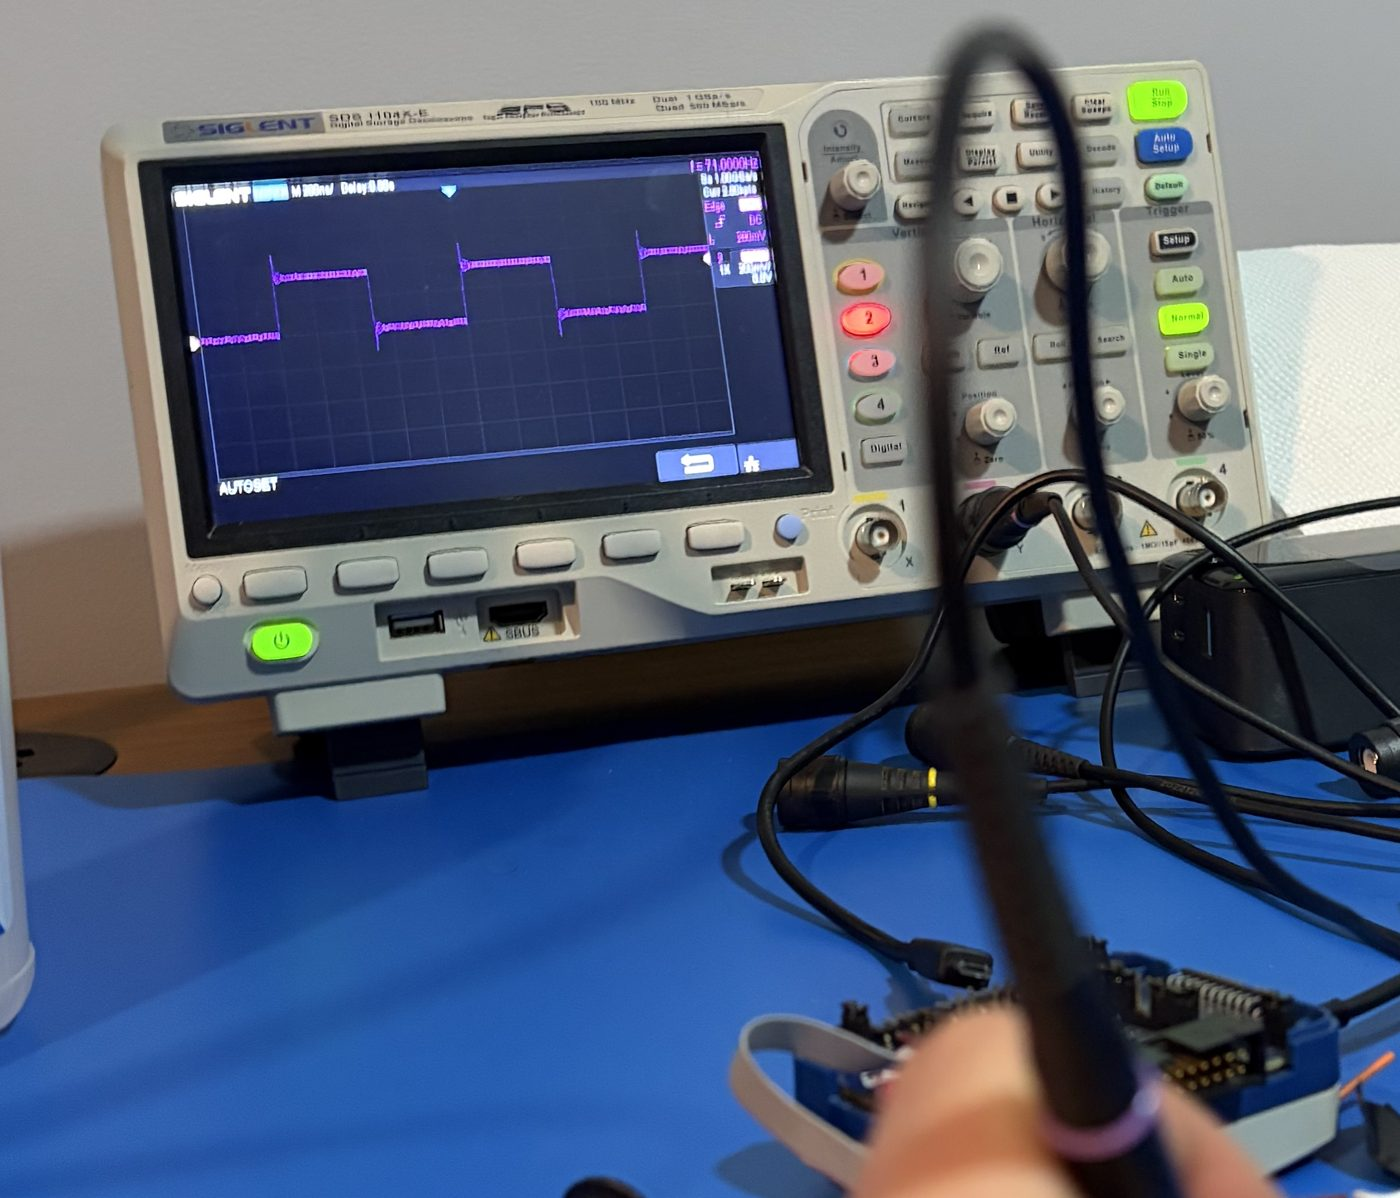
\includegraphics[height=1.62in]{figs/qspi_clk_probe.jpg}
  \caption{Verifying QSPI clock at the flash.}
\end{subfigure}\hfill
\begin{subfigure}[t]{2.69in}\centering
  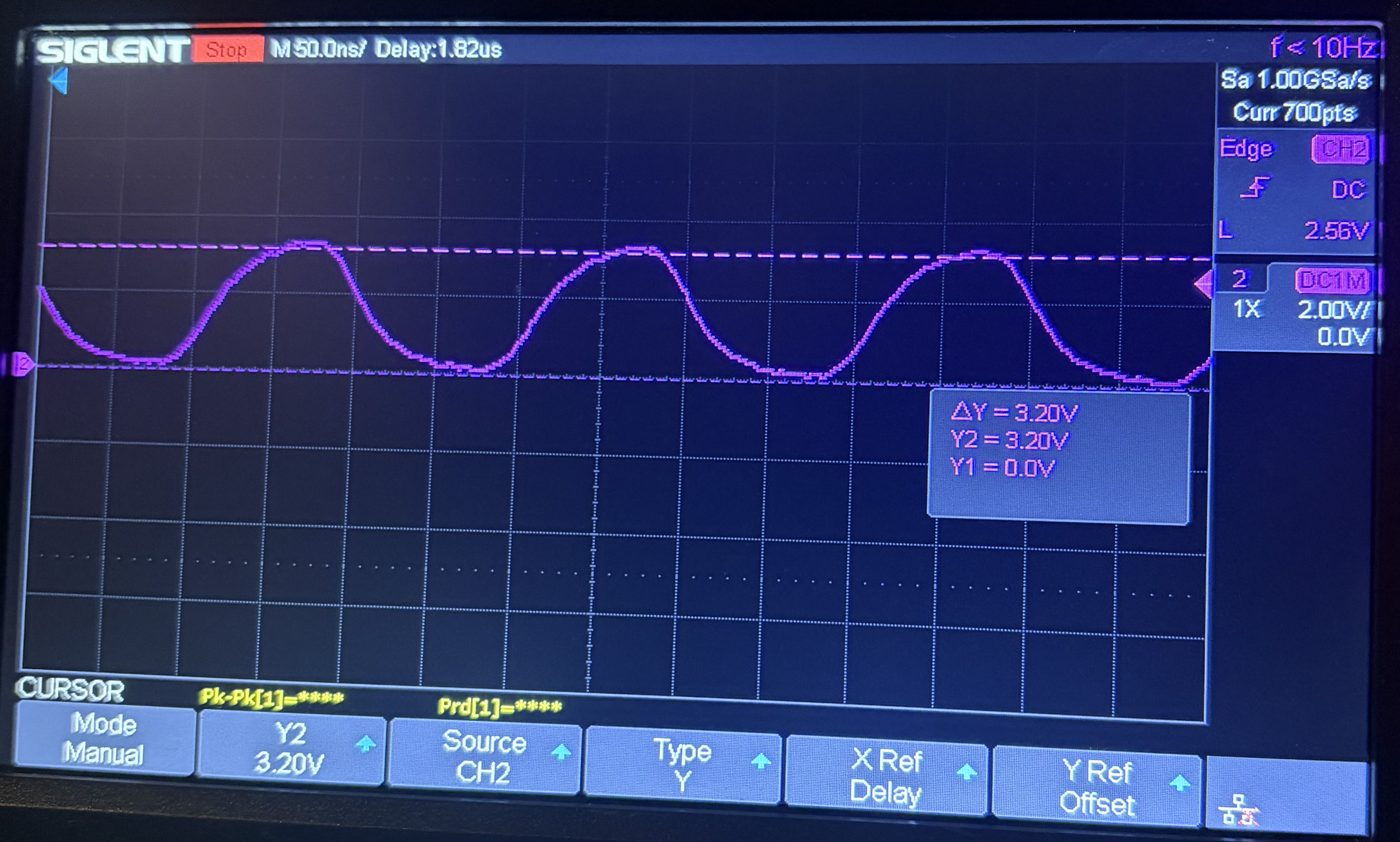
\includegraphics[height=1.62in]{figs/spi_5mhz_clk.jpg}
  \caption{Sensor SPI clock at 5 MHz.}
\end{subfigure}
\caption{Oscilloscope-driven debugging of the QSPI flash and sensor SPI bus.}
\end{figure}


%-------------------------------------------------------------------------------
\section{Embedded Software}
C on STM32's hardware abstraction layer, built with CMake \& STM32CubeIDE. Drivers share one lifecycle,
\texttt{AssignSPI} (bind bus and chip select, no bus traffic) $\to$ \texttt{Init(dev, \&config)}
(validate, copy, configure) $\to$ blocking reads, documented in a short API guide so
teammates can add sensors consistently.

\textbf{How I built the drivers.} I read the datasheets to design the SPI register access layer
(read-bit framing, chip-select handling, multi-byte reads) and the driver structure, then used
AI tooling to fill in register-level configuration options. I treated generated code as
untrusted until validated on hardware.

\textbf{Defensive design (R4).} Nothing reaches the application unless it is validated:
\begin{itemize}
\item \textbf{Configuration:} invalid output-rate or full-scale values are rejected before any
  bus traffic; drivers copy configuration so callers cannot change it underneath them; a failed
  \texttt{Init} always clears the \texttt{initialized} flag, and reads fail until it succeeds.
\item \textbf{MS5611 barometer:} the sensor has no ID register, so startup reads its 8 factory
  calibration words and checks their CRC-4, and rejects all-zero/all-one values typical of a
  disconnected bus. Pressure compensation (including second-order low-temperature terms) uses
  signed 64-bit integer math, and conversion waits use the datasheet's worst-case timings.
\item \textbf{IMU:} block-data-update is enabled so high and low bytes always come from the same
  sample; WHO\_AM\_I must match before configuration.
\end{itemize}

\textbf{Attitude estimation (R5).} A complementary filter at 50~Hz propagates roll $\phi$ and
pitch $\theta$ with the Euler-angle kinematics and corrects slowly toward the
accelerometer's gravity tilt ($\alpha = 0.05$):
% \[
% \dot\phi = p + \tan\theta\,(q\sin\phi + r\cos\phi),\qquad
% \dot\theta = q\cos\phi - r\sin\phi,\qquad
% \hat x_k = (1-\alpha)\,(\hat x_{k-1} + \dot x\,\Delta t) + \alpha\, x_{\text{acc}}.
% \]

\[
\begin{bmatrix}
    \dot{\phi} \\
    \dot{\theta}
\end{bmatrix}
=
\begin{bmatrix}
    1 & \sin(\phi)\tan(\theta) & \cos(\phi)\tan(\theta) \\
    0 & \cos(\phi)             & -\sin(\phi)
\end{bmatrix}
\begin{bmatrix}
    p \\
    q \\
    r
\end{bmatrix}
\]

\[
\hat{\phi}_{n+1}
=
\hat{\phi}_{\mathrm{acc},n}\cdot\alpha
+
(1-\alpha)\cdot
\left[
    \hat{\phi}_n + T\cdot\dot{\phi}_{\mathrm{gyr},n}
\right]
\]
where $T$ is the measured interval between samples (nominally 20~ms) and $\dot{\phi}_{\mathrm{gyr},n}$
comes from the kinematics above. Pitch $\hat{\theta}$ is updated analogously; roll is additionally
wrapped to $\pm180^\circ$.

The current filter is not intended for flight, but is a learning step towards developing a Kalman filter which is capable of 
handling actual flight. Edge cases are handled explicitly: 
non-finite or zero samples are rejected; the filter re-seeds from the accelerometer after a timing gap above 250~ms; 
roll correction takes the shortest path across $\pm180^\circ$; and near $\theta=\pm90^\circ$, where these 
Euler rates are singular, it falls back to accelerometer tilt. Output streams as CSV over SWO for later analysis.

%-------------------------------------------------------------------------------
\section{Verification}
\begin{minipage}[t]{0.52\textwidth}
\vspace{0pt}
\textbf{Host unit tests.} The real driver sources compile on a PC against a mock HAL that
simulates the sensor's registers and asserts bus behavior on every call:
\begin{itemize}
\item MS5611 math matches the datasheet's worked example (1000.09~mbar, 20.07~$^\circ$C),
  plus low and very-low temperature compensation and CRC-4.
\item Protocol: chip-select is low for every transfer and high during conversion delays;
  command framing and every OSR delay are correct.
\item Fault injection: SPI timeouts, zero ADC data, corrupt or blank calibration PROM, and
  invalid configurations each return the right error; a failed \texttt{Init} leaves
  \texttt{initialized} cleared.
\end{itemize}
\textbf{On hardware.} Each sensor ID and the flash JEDEC ID are checked at startup and
reported over SWO. Bench tests (right) show the filter tracking deliberate rolls and pitches of the board.
\end{minipage}\hfill
\begin{minipage}[t]{0.45\textwidth}
\vspace{0pt}
\centering
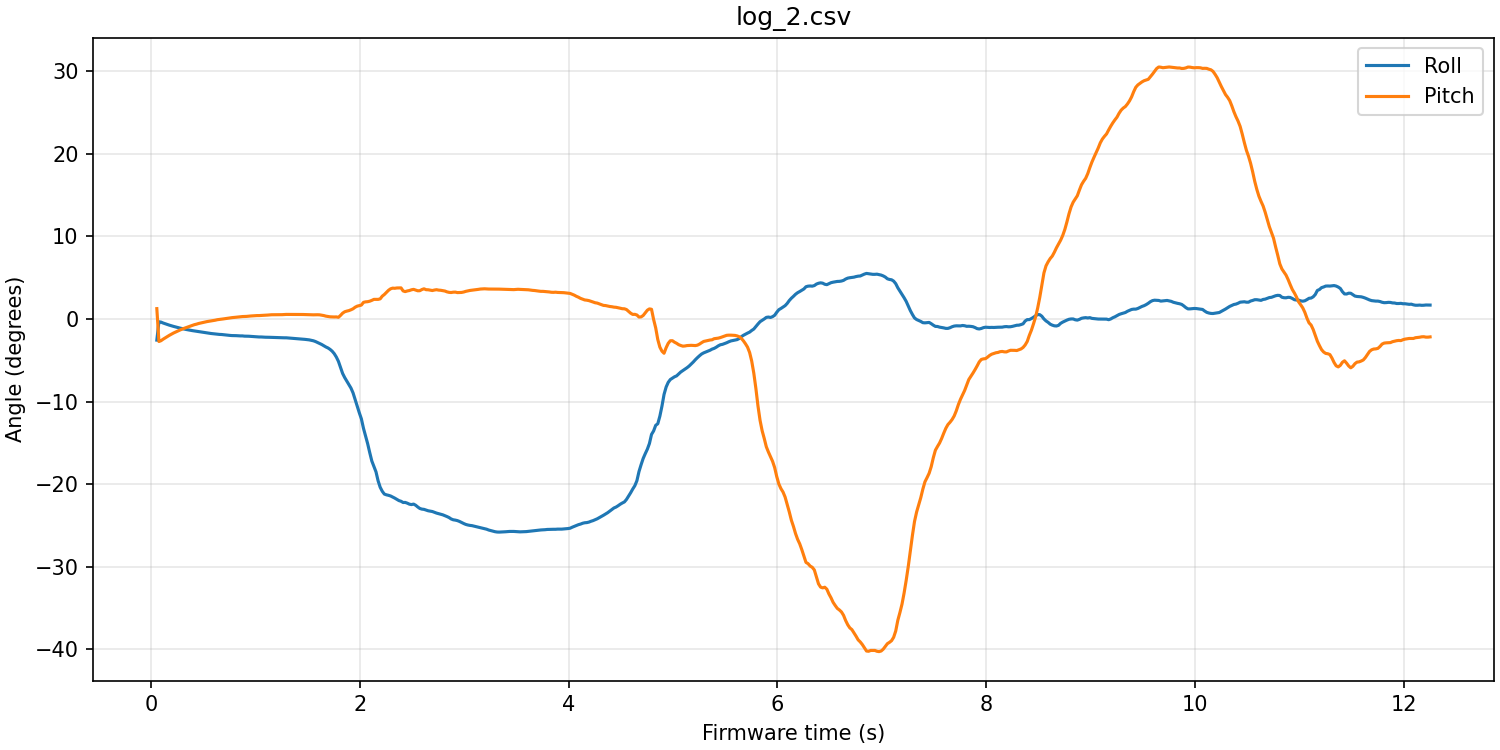
\includegraphics[width=\linewidth]{figs/bench_attitude.png}
\captionof{figure}{Bench test: roll ($\approx -25^\circ$) then pitch ($-40^\circ$/$+30^\circ$)
  maneuvers, logged over SWO at 50 Hz.}
\end{minipage}

%-------------------------------------------------------------------------------
\section{Status, Known Limitations, and Next Steps}

\textbf{Currently working:} power, clocks, SWD/SWO, and the ASM330LHHX and MS5611 drivers. The ADXL375 driver was proven, then the part was removed. Flash logging awaits the replacement flash, and the MMC5983 is not yet working. Current limitations:
\begin{itemize}
\item \textbf{Accelerometer correction under thrust:} During boost the accelerometer measures
  thrust plus gravity, so the tilt correction is invalid. Boost needs a different tilt reference,
  such as gyro-only propagation with magnetometer aiding.
\item \textbf{Range:} The ASM330LHHX is configured at $\pm2$~g for bench work; flight needs
  $\pm16$~g plus the high-g sensor restored in rev~B (R3).
\item \textbf{Scheduling:} A 20~ms blocking barometer read conflicts with the 20~ms IMU loop, so
  state estimation cannot yet run at a fixed $\Delta t$ (addressed in roadmap phase~2).
\item \textbf{Axis convention:} The sensor-to-board axis mapping is currently a reflection
  (left-handed) and must become a proper rotation matching the silkscreen axes.
\item \textbf{Traceability:} Finish the requirements document with a table linking each
  requirement to its verification.
\end{itemize}
\textbf{Roadmap:} Each phase ends with a verification gate that must pass before the next begins.

\vspace{2pt}
{\small
\renewcommand{\arraystretch}{1.15}
\begin{tabularx}{\linewidth}{@{}c>{\raggedright\arraybackslash}p{0.17\linewidth}>{\raggedright\arraybackslash}X>{\raggedright\arraybackslash}p{0.07\linewidth}>{\raggedright\arraybackslash}p{0.29\linewidth}@{}}
\toprule
& \textbf{Phase} & \textbf{Work} & \textbf{Req.} & \textbf{Passing criterion} \\
\midrule
1 & Flash logging &
  Replace W25Q128JV; QSPI page-program driver with DMA; log frame format and host read-back tool. &
  R1, R2 &
  $\geq 420$~s of frames logged on the bench and read back intact. \\
2 & Real-time firmware &
  FreeRTOS tasks; IMU data-ready interrupts; non-blocking barometer state machine; host tests in CI. &
  R1, R4 &
  Fixed $\Delta t$ confirmed with LED/scope timing; logging continues with a sensor disconnected. \\
3 & Flight readiness &
  $\pm16$~g IMU range; correct sensor-to-board axis rotation; gate accel correction under thrust. &
  R3, R5 &
  Tilt tests match silkscreen axes; simulated boost profile does not corrupt attitude. \\
4 & L2 flight (J270) &
  Fly Melchior as a passive logger alongside a commercial altimeter. &
  R1--R5 &
  Full flight log recovered; on-board estimate compared against post-flight analysis. \\
5 & Rev~B and Kalman filter &
  ADXL375 SDA isolation gate; routing and SPI timing margin; Kalman filter tuned on flight logs. &
  R3, R5 &
  High-g data on a shared bus without errors; filter validated against recorded flight. \\
6 & Pyro and power board &
  Separate board with battery protection, buck regulation, and pyro channels. &
  R6 &
  Independent verification before any pyro channel flies. \\
\bottomrule
\end{tabularx}}

\end{document}
